%\section{{\em k-}iteration Path Profiling}
\section{Multi-iteration Path Profiling}

In this section, we discuss and evaluate an implementation, which we call \kblpp, of our approach to multi-iteration path profiling in the Jikes Research Virtual Machine (RVM)~\cite{Alpern00}. Our code is publicly available in the Jikes RVM Research Archive\footnote{\url{http://sourceforge.net/p/jikesrvm/research-archive/41/}.} and has been endorsed by the OOPSLA 2013 Artifact Evaluation Committee. The goal of our experimental study is to assess the performance of our profiler compared to previous approaches and to study properties of path profiles that span multiple iterations for several representative benchmarks. The results indicate that our technique can profile paths that extend across many loop iterations in a time comparable with acyclic path profiling on a large variety of industry-strength benchmarks.

\subsection{Implementation}

\paragraph*{Adaptive Compilation.} The Jikes RVM is a high-performance {\em meta-circular} virtual machine: unlike most other JVMs, it is written in Java. The Jikes RVM does not include an interpreter: all bytecode must be first translated into native machine code. The unit of compilation is the method, and methods are compiled lazily by a fast non-optimizing compiler -- the so-called {\em baseline} compiler -- when they are first invoked by the program. As execution continues, the Adaptive Optimization System monitors program execution to detect program hot spots and selectively recompiles them with three increasing levels of optimization. This approach is typical of modern production JVMs, which rely on some variant of selective optimizing compilation to target the subset of the hottest program methods where they are expected to yield the most benefits.

Recompilation is performed by the {\em optimizing} compiler, that generates higher-quality code but at a significantly larger cost than the baseline compiler. Since Jikes RVM quickly recompiles frequently executed methods, we implemented \kblpp in the optimizing compiler only.

\paragraph*{Adding Instrumentation.} As discussed in \mysection\ref{ss:kblpp-approach}, the Ball-Larus tracing technique requires instrumenting CFG edges so that when an edge is traversed, the probe value is incremented by a quantity computed by the path numbering algorithm on the DAG obtained by transforming back edges in the CFG.

\kblpp\ adds instrumentation to hot methods in three passes:
\begin{enumerate}[itemsep=0pt]
 \item building the DAG representation;
 \item assigning values to edges;
 \item adding instrumentation to edges.
\end{enumerate}

\noindent \kblpp\ adopts the {\em smart path numbering} algorithm proposed by Bond and McKinley~\cite{Bond05b} to improve performance by placing instrumentation on cold edges. In particular, line 6 of the canonical Ball-Larus path numbering algorithm shown in \myalgorithm\ref{alg:kblpp-bl-numbering} \ifauthorea{}{(page \pageref{alg:kblpp-bl-numbering})} is modified such that outgoing edges are picked in decreasing order of execution frequency. For each basic block edges are sorted using existing edge profiling information collected by the baseline compiler: we can thus assign zero to the hottest hedge, so that \kblpp\ will not place any instrumentation on it.
%in this way we can assign zero to the hottest edge, thus allowing us to assign zero to the hottest edge so that \kblpp\ does not place any instrumentation on it.

During compilation, the Jikes RVM introduces {\em yield points}, which are program points where the running thread determines if it should yield to another thread. Since JVMs need to gain control of threads quickly, compilers insert yield points in method prologues, loop headers, and method epilogues. We modified the optimizing compiler to also store the path profiling probe on loop headers and method epilogues. Ending paths at loop headers rather than back edges causes a path that traverse a header to be split into two paths: this difference from canonical Ball-Larus path profiling is minor because it only affects the first path through a loop~\cite{Bond05}.

Note that optimizing compilers do not insert yield points in a method when either it does not contain branches (hence its profile is trivial) or it is marked as uninterruptible. The second case occurs in internal Jikes RVM methods only; the compiler occasionally inlines such a method into an application method, and this might result in a loss of information only when the execution reaches a loop header contained in the inlined method. However, according to \cite{Bond05}, this loss of information appears to be negligible.

\paragraph*{Path Profiling.} To make fair performance comparisons with state-of-the-art previous profilers, we built our code on top of the BLPP profiler developed by Bond~\cite{Bond05,PEP}, which provides an efficient implementation of the Ball-Larus acyclic-path profiling technique. The \ksf\ construction algorithm described in \mysection\ref{ss:kblp-algorithms} is implemented using a standard first-child, next-sibling representation for nodes. This representation is very space-efficient, as it requires only two pointers per node: one to its leftmost child and the other to its right nearest sibling. % - while experimental results show that the average degree of a node is usually low.

\ifdefined\noauthorea
\begin{figure}[!ht]
\begin{center}
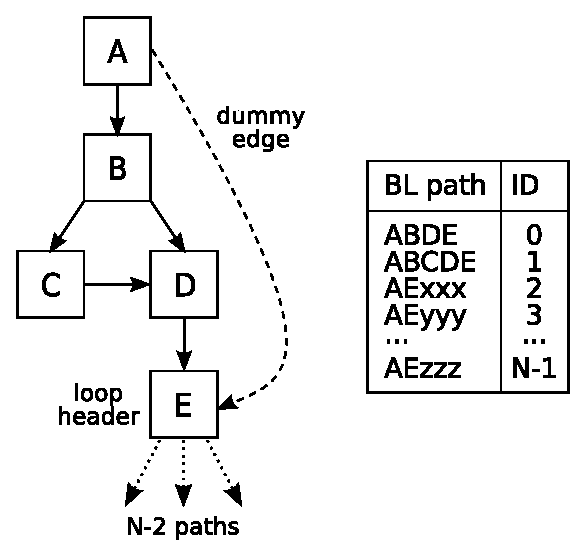
\includegraphics[width=0.4\textwidth]{figures/kblpp-example-fewer/kblpp-example-fewer.eps}
\caption{\protect\label{fig:kblpp-example-fewer} Routine with an initial branch before the first cycle.}
\end{center}
\end{figure}
\fi

\noindent Tree roots are stored and accessed through an efficient implementation\footnote{{\tt HashMapRVM} is a stripped-down implementation of the {\tt HashMap} data structure used by core parts of the Jikes RVM runtime and by Bond's BLPP path profiler.} of a hash map, using the pair represented by the Ball-Larus path ID and the unique identifier associated to the current routine (i.e., the compiled method ID) as key. Note that this map is typically smaller than a map required by a traditional BLPP profiler, since tree roots represent only a fraction of the distinct path IDs encountered during the execution. Consider, for instance, the example shown in \myfigure\ref{fig:kblpp-example-fewer}: this control flow graph has $N$ acylic paths after backedges have been removed. Since cyclic paths are truncated on loop headers, only path IDs $0$ and $1$ can appear after the special marker $*$ in the stream, thus leading to the creation of an entry in the hash map. Additional entries might be created when a new tree is added to the \ksf\ (line 10 of the streaming algorithm shown in \myalgorithm\ref{alg:kblpp-ksf-algorithm}\ifauthorea{}{ on page \pageref{alg:kblpp-ksf-algorithm}}); however, experimental results show that the number of tree roots is usually small, while $N$ increases with the complexity (i.e., number of branches and loops) of the routine.

\subsection{Experimental Setup}

In this section we illustrate the details of our experimental methodology, focusing on benchmarks, performance and topological metrics, and compared profiling techniques.

\subsubsection*{Benchmarks}

We evaluated \kblpp\ against a variety of prominent benchmarks drawn from three suites. The \dacapo\ suite~\cite{Blackburn06} consists of a set of open source, real-world applications with non-trivial memory loads. We use the superset of all benchmarks from \dacapo\ releases 2006-10-MR2 and 9.12 that can run successfully in the Jikes RVM, using the largest available workload for each benchmark. In particular, {\tt avrora}, {\tt jython}, {\tt luindex}, {\tt sunflow}, and {\tt xalan} are taken from the 9.12 release, while {\tt chart}, {\tt eclipse}, and {\tt hsqldb} are from the 2006-10-MR2 release.

The \specjvm\ suite focuses on the performance of the hardware processor and memory subsystem when executing common general purpose application computations. Benchmarks from the suite that can run successfully\footnote{Due to limitations of the GNU classpath, only a small number of them are supported.} on the Jikes RVM include: {\tt compiler.compiler}, {\tt compress}, {\tt mpegaudio}, and {\tt scimark.\{montecarlo, sor.large, sparse.large\}}.

Finally, we chose two memory-intensive benchmarks ({\tt heapsort} and {\tt md}) from the \javagrande\ $2.0$ suite~\cite{Bull99} to further evaluate the performance of \kblpp.

\subsubsection*{Metrics}
We considered a variety of metrics, including wall-clock time, number of operations per second performed by the profiled program, number of hash table operations, data structure size (e.g., number of hash table items for \blpp\ and number of \ksf\ nodes for \kblpp), and statistics such as average node degree of the \ksf\ and the \kipf\ and average depth of \kipf\ leaves. To interpret our results, we also ``profiled our profiler'' by collecting hardware performance counters with {\tt perf}~\cite{perf}, including L1 and L2 cache miss rate, branch mispredictions, and cycles per instruction (CPI).

\subsubsection*{Compared Codes}
In our experiments, we analyzed the native (uninstrumented) version of each benchmark and its instrumented counterparts, comparing \kblpp\ for different values of $k$ (2, 3, 4, 6, 8, 11, 16) with the \blpp\ profiler developed by Bond~\cite{PEP} for Ball-Larus acyclic-path profiling. We upgraded the original tool by Bond to take advantage of native threading support introduced in later Jikes RVM releases; the code is structured as in \myfigure\ref{fig:kblpp-approach}\ifauthorea{}{ (page \pageref{fig:kblpp-approach})}, except that it does not produce any intermediate stream, but it directly performs {\tt count[r]++}.

\subsubsection*{Platform}
Experiments were performed on a 2.53GHz Intel Core2 Duo T9400 with 128KB of L1 data cache, 6MB of L2 cache, and 4 GB of main memory DDR3 1066, running Ubuntu 12.10, Linux Kernel 3.5.0, 32 bit. We ran all of the benchmarks on Jikes RVM 3.1.3 (default {\tt production} build) using a single core and a maximum heap size equal to half of the amount of physical memory. For each benchmark/profiler combination, we performed 10 trials, each preceded by a warmup execution, and computed the arithmetic mean. Performance measurements were collected on a machine with negligible background activity. We report confidence intervals stated at 95\% confidence level.

\subsection{Time Overhead}

In \myfigure\ref{fig:kblpp-slowdown} we report for each benchmark the profiling overhead of \kblpp\ relative to \blpp. The chart shows that for 12 out of 16 benchmarks the overhead decreases for increasing values of $k$, providing up to almost 45\% improvements over \blpp. This is explained by the fact that hash table accesses are performed by {\tt process\_bl\_path\_id} every $k-1$ items read from the input stream between two consecutive routine entry events (lines 8 and 10 in \myalgorithm\ref{alg:kblpp-ksf-algorithm}\ifauthorea{)}{on page \pageref{alg:kblpp-ksf-algorithm})}. As a consequence, the number of hash table operations for each routine call is $O(1+N/(k-1))$, where $N$ is the total length of the path taken during the invocation.

\ifdefined\noauthorea
\begin{figure}[!ht]
\begin{center}
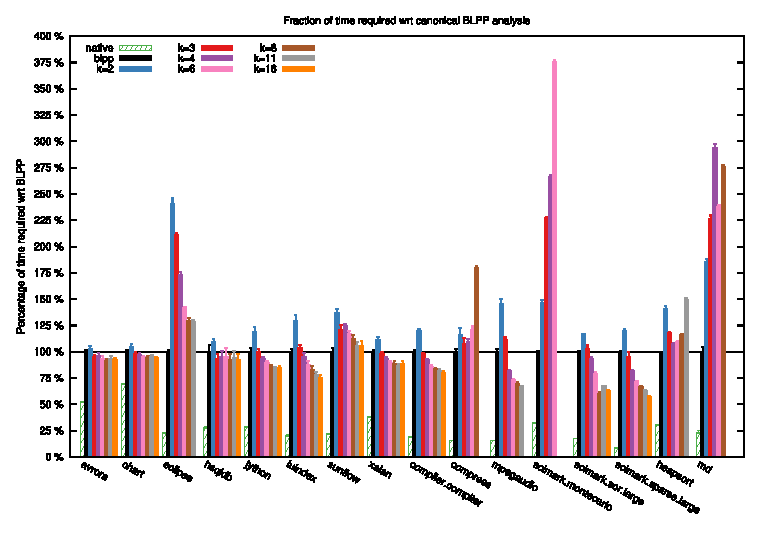
\includegraphics[width=\textwidth]{figures/kblpp-slowdown/kblpp-slowdown.eps}
\caption{\protect\label{fig:kblpp-slowdown} Performance of \kblpp\ relative to \blpp.
}
\end{center}
\end{figure}
\fi

In \myfigure\ref{fig:kblpp-hash} we report the measured number of hash table accesses for our experiments, which decreases as predicted on all benchmarks with intense loop iteration activity. Notice that, not only does \kblpp\ perform fewer hash table operations, but since only a subset of BL path IDs are inserted, the table is also smaller yielding further performance improvements. For codes such as {\tt avrora} and {\tt hsqldb}, which perform on average a small number of iterations, increasing $k$ beyond this number does not yield any benefit.

\ifdefined\noauthorea
\begin{figure}[!ht]
\begin{center}
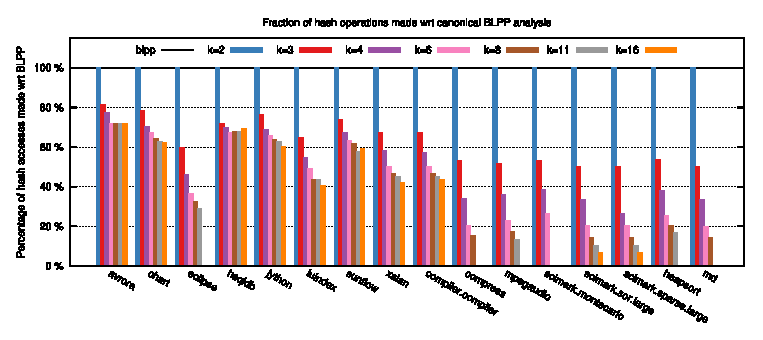
\includegraphics[width=\textwidth]{figures/kblpp-hash/kblpp-hash.eps}
\caption{\protect\label{fig:kblpp-hash} Number of hash table operations performed by \kblpp\ relative to \blpp.
}
\end{center}
\end{figure}
\fi

On {\tt eclipse}, \kblpp\ gets faster as $k$ increases, but differently from all other benchmarks in this class, it remains slower than \blpp\ by at least 25\%. The reason is that, due to structural properties of the benchmark, the average number of node scans at lines 13 and 21 of {\tt process\_bl\_path\_id} is rather high (58.8 for $k=2$ down to 10.3 for $k=16$). In contrast, the average degree of internal nodes of the \ksf\ is small (2.6 for $k=2$ decreasing to 1.3 for $k=16$), hence there is intense activity on nodes with a high number of siblings. No other benchmark exhibited this extreme behavior. We expect that a more efficient implementation of {\tt process\_bl\_path\_id}, e.g., by adaptively moving hot children to the front of the list, could reduce the scanning overhead for this kind of worst-case benchmarks as well.

Benchmarks {\tt compress}, {\tt scimark.montecarlo}, {\tt heapsort}, and {\tt md} made an exception to the general trend we observed, with performance overhead increasing, rather than decreasing, with $k$. To justify this behavior, we collected and analyzed several hardware performance counters and noticed that on these benchmarks our \kblpp\ implementation suffers from increased CPI for higher values of $k$.

\ifdefined\noauthorea
\begin{figure}[!ht]
\begin{center}
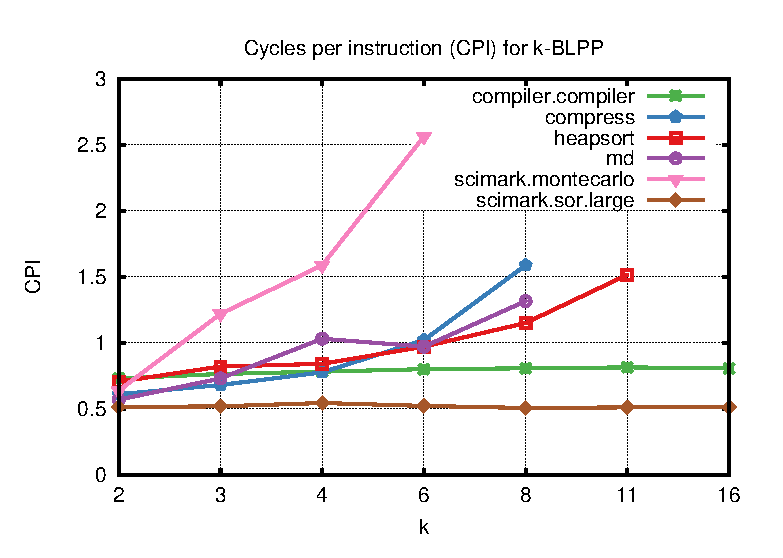
\includegraphics[width=0.49\textwidth]{figures/kblpp-cpi/kblpp-cpi.eps}
\caption{\protect\label{fig:kblpp-cpi} Hardware performance counters for \kblpp: cycles per instruction (CPI).
}
\end{center}
\end{figure}
\fi

\myfigure\ref{fig:kblpp-cpi} shows this phenomenon, comparing the four outliers with other benchmarks in our suite. By analyzing L1 and L2 cache miss rates, reported in \myfigure\ref{fig:kblpp-cache} (a) and \myfigure\ref{fig:kblpp-cache} (b), we noticed that performance degrades due to poor memory access locality. We believe this to be an issue of our current implementation of \kblpp, in which we did not make any effort aimed at improving cache efficiency in accessing the \ksf, rather than a limitation of the general approach we propose. Indeed, as nodes may be unpredictably scattered in memory due to the linked structure of the forest, pathological situations may arise where node scanning incurs several cache misses.

\ifdefined\noauthorea
\begin{figure}[!ht]
\begin{center}
\begin{tabular}{cc}
\hspace{-6mm}
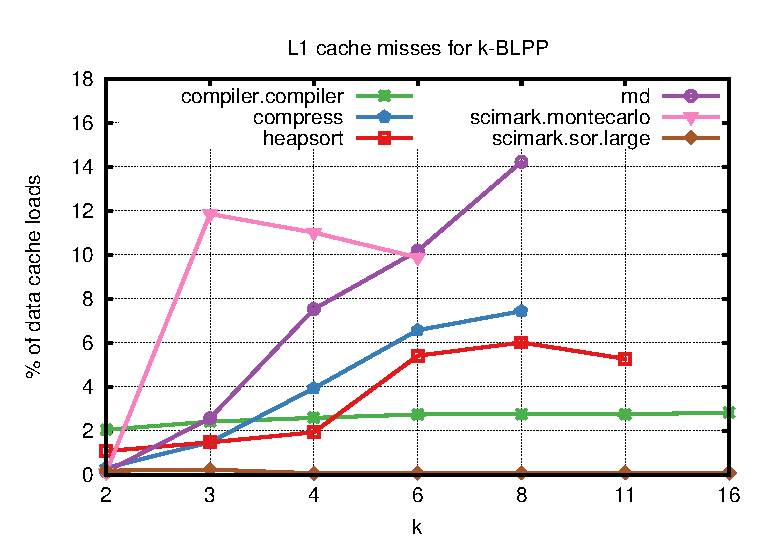
\includegraphics[width=0.49\textwidth]{figures/kblpp-cache/kblpp-cache-L1.eps} &
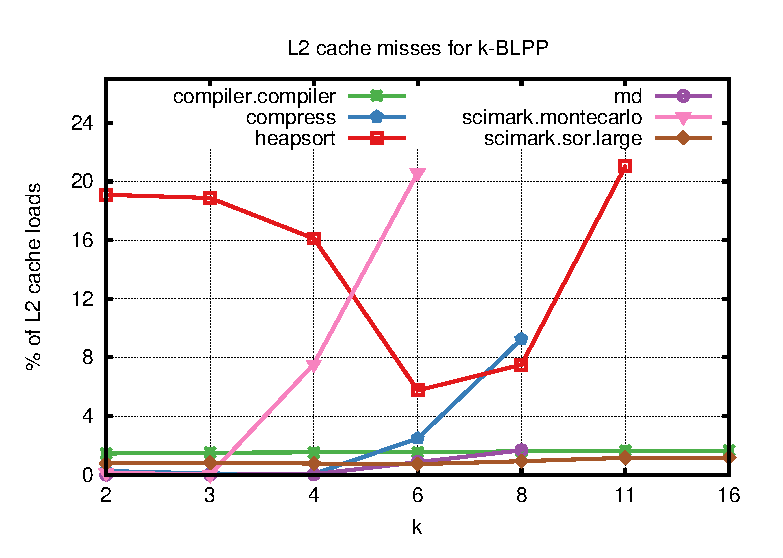
\includegraphics[width=0.49\textwidth]{figures/kblpp-cache/kblpp-cache-L2.eps}\\
(a) & (b)
\end{tabular}
\caption{\protect\label{fig:kblpp-cache} Hardware performance counters for \kblpp: (a) L1 and (b) L2 cache miss rates.}
\end{center}
\end{figure}
\fi

Notice that, since we never delete either entries from the hash table or nodes from the \ksf, our implementation does not place any additional burden on the garbage collector. The profiler causes memory release operations only when a thread terminates, dumping all of its data structures at once.

\subsection{Memory Usage and Structural Properties}
\myfigure\ref{fig:kblpp-space} compares the space requirements of \blpp\ and \kblpp\ for different values of $k$. The chart reports the total number of items stored in the hash table by \blpp\ and the number of nodes in the \ksf.

\ifdefined\noauthorea
\begin{figure}[!ht]
\begin{center}
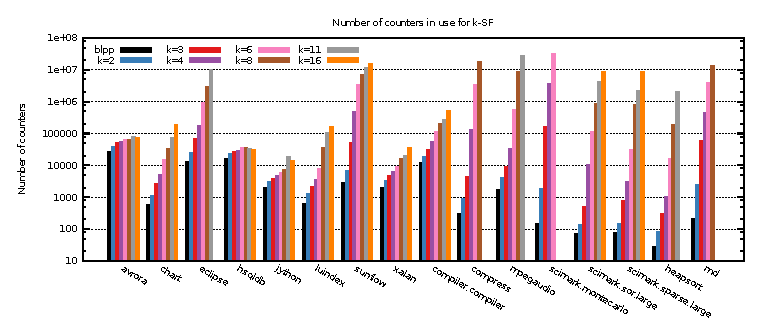
\includegraphics[width=\textwidth]{figures/kblpp-space/kblpp-space.eps}
\caption{\protect\label{fig:kblpp-space} Space requirements: number of hash table entries in \blpp\ and number of nodes in the \ksf.

}
\end{center}
\end{figure}
\fi

Since both \blpp\ and \kblpp\ exhaustively encode exact counters for all distinct taken paths of bounded length, space depends on intrinsic structural properties of the benchmark. Programs with intense loop iteration activity are characterized by substantially higher space requirements by \kblpp, which collects profiles containing up to several millions of paths. Notice that on some benchmarks we ran out of memory for large values of $k$, hence some bars in the charts we report in this section are missing. In \myfigure\ref{fig:kblpp-space-kipf} we report the number of nodes in the \kipf, which corresponds to the number of paths profiled by \kblpp. Notice that, since a path may be represented more than once in the \ksf, the \kipf\ represents a more compact version of the \ksf.

\ifdefined\noauthorea
\begin{figure}[!ht]
\begin{center}
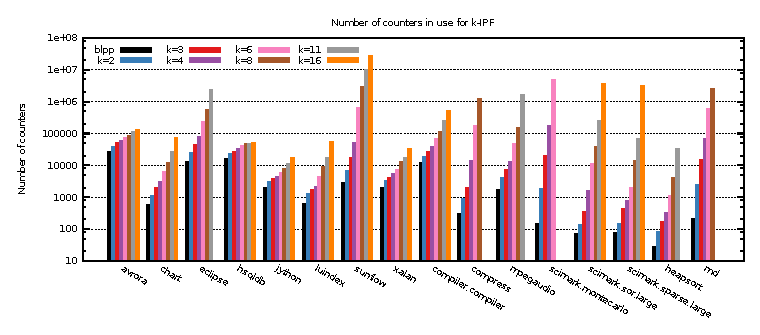
\includegraphics[width=\textwidth]{figures/kblpp-space-kipf/kblpp-space-kipf.eps}
\caption{\protect\label{fig:kblpp-space-kipf} Number of paths profiled by \blpp\ and \kblpp.

}
\end{center}
\end{figure}
\fi

\ifdefined\noauthorea
\begin{figure}[!ht]
\begin{center}
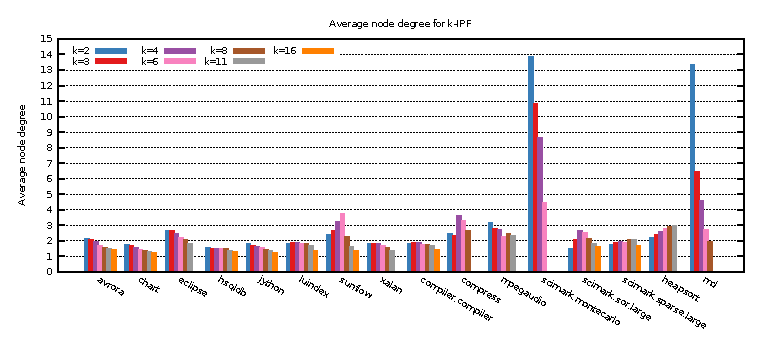
\includegraphics[width=\textwidth]{figures/kblpp-kipf-degree/kblpp-kipf-degree.eps}
\caption{\protect\label{fig:kblpp-kipf-degree} Average degree of \kipf\ internal nodes.

}
\end{center}
\end{figure}
\fi

As a final experiment, we measured structural properties of the \kipf\ such as average degree of internal nodes (\myfigure\ref{fig:kblpp-kipf-degree}) and the average leaf depth (\myfigure\ref{fig:kblpp-kipf-leaves}). Our tests reveal that the average node degree generally decreases with $k$, showing that similar patterns tend to appear frequently across different iterations. Some benchmarks, however, such as {\tt sunflow} and {\tt heapsort} exhibit a larger variety of path ramifications, witnessed by increasing node degrees at deeper levels of the \kipf. The average leaf depth allows us to characterize the loop iteration activity of different benchmarks. Notice that for some benchmarks, such as {\tt avrora} and {\tt hsqldb}, most cycles consist of a small number of iterations: hence, by increasing $k$ beyond this number, \kblpp\ does not collect any additional useful information.

\ifdefined\noauthorea
\begin{figure}[!ht]
\begin{center}
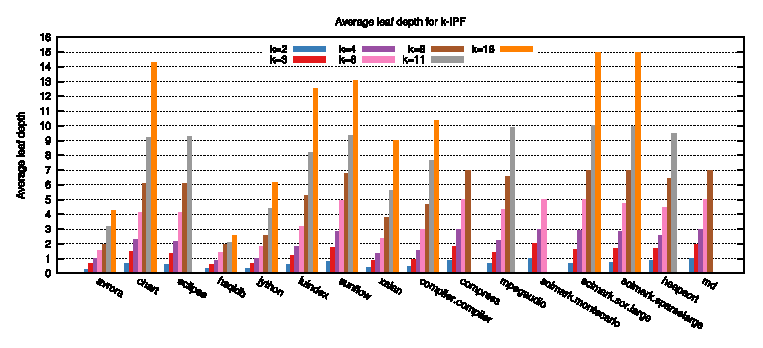
\includegraphics[width=\textwidth]{figures/kblpp-kipf-leaves/kblpp-kipf-leaves.eps}
\caption{\protect\label{fig:kblpp-kipf-leaves} Average depth of \kipf\ leaves.

}
\end{center}
\end{figure}
\fi